\documentclass[10pt, a4paper]{IEEEtran}
\usepackage[T1]{fontenc}
\usepackage{mathtools}
\usepackage[usenames,dvipsnames]{color}
\usepackage{parskip}
\setlength{\parskip}{0pt}
\setlength{\parindent}{15pt} 
\usepackage{multirow}
\usepackage{amsfonts}
\usepackage{amssymb}
\usepackage{booktabs}
\usepackage{listings}
\usepackage[justification=centering]{caption}
\usepackage{pgfplots}
\title{Software Optimizations for Reduced CPU Energy Consumption: A Feasibility Study}                            
\author{\IEEEauthorblockN{Stephen I. Roberts and Stephen Jarvis} \\
\IEEEauthorblockA{Department of Computer Science,\\
The University of Warwick}\\
\and 
\IEEEauthorblockN{Chris January and Jonathan Byrd} \\
\IEEEauthorblockA{Allinea Software}}                                                            

\hyphenation{scaling}

\newcommand{\golden}{}
%\renewcommand{\golden}{{\color{green} \checkmark}}


\newcommand{\findref}{}
\renewcommand{\findref}{{\color{red} FindRef}}

\newcommand{\todo}[1]{}
\renewcommand{\todo}[1]{{\color{red} TODO: {#1}}} % comment me out for prod

\newcommand{\reword}[1]{}
\renewcommand{\reword}[1]{{\color{blue} Reword: {#1}}} %

\newcommand{\fragment}[1]{}
\renewcommand{\fragment}[1]{{\color{green}<fragment>}{#1}{\color{green}</fragment>}} %

\makeatletter
\newcommand{\choice}[2][ |]{{\color{Purple}\{%
  \def\nextitem{\def\nextitem{#1}}%
  \@for \el:=#2\do{\nextitem\el}%
\}}}
\makeatother

\begin{document}                                                                
\maketitle

\begin{abstract}
Reducing energy consumption is a prerequisite for future advances in computing at scale. This fact has led performance engineers to explore software-level power optimization as a potential means to reduce the energy consumed by scientific codes. Our work investigates the feasibility and potential benefits of this approach. We present a simple visual heuristic which allows energy conscious developers to decide whether to focus their efforts on runtime or power optimization. We then attempt to provide a realistic impression about how much arbitrary codes may benefit from power optimizations. Our work concludes by investigating how useful current methods are when searching for power optimizations. We find that for current hardware there is limited scope for improving energy efficiency through software power optimisation alone. \golden
\end{abstract}

\section*{Introduction}
Driven by Moore's Law, advances in processor design have delivered improvements in CPU performance for decades. As physical limits are reached, however, refinements to the same basic technologies are beginning to show diminishing returns. One side-effect of this is an unsustainable rise in system power usage, which the US Department of Energy has identified as a primary constraint for exascale systems \cite{shalf:2011aa}.

Hardware manufacturers are already prioritising energy efficiency in their processor designs~\cite{kurd:2014aa}. In turn, some groups have suggested that software modifications will be required to fully exploit the energy efficiency improvements of modern processors~\cite{shao:2013aa}. This is analogous to the current practice of tuning code for reduced runtime by exploiting specific processor features like vectorisation or cache hierarchy. These groups expect targeted optimisation to be applied to reducing power consumption in the future.

A body of research is accumulating as the search for techniques to identify and reason about software power optimizations continues. The intent of this paper is to provide a critical review of the field; identifying the opportunities present and highlighting the amount of benefit which can be realistically expected of them. We approach this task in two ways. Firstly we review the prior art in this field to identify any trends and secondly we provide an empirical investigation, applying some of the proposed techniques in order to understand how they may benefit developers.

The remainder of this paper is organized as follows: Section~\ref{sec:background} details the problem background and introduces some core concepts and metrics. Section~\ref{sec:prior} gives an overview of prior research carried out in this area. Section~\ref{sec:profiling} then investigates how the techniques described in Section~\ref{sec:prior} may be applied practically.\todo{finish, condense}

\section{Background}
\label{sec:background}
Despite recent interest, concerns about system power have existed since the dawn of computing. Some of the earliest valve-based computers had power draws comparable to modern supercomputers. The ENIAC machine dissipated 174 kW \cite{birnbaum:2000aa}, a figure which would not look out of place in the current Top 500 list, despite the fact this machine dates from 1947.\golden

When bipolar semiconductor technologies superseded thermionic valves in the 1950s and 60s the result was a dramatic reduction in system power consumption. Over time, manufacturing improvements delivered ever smaller transistors, yielding rapid increases in both performance and power density. Ultimately this resulted in chips which strained the limits of cooling technologies~\cite{jouppi:1994aa}. \golden

The use of bipolar semiconductors peaked in the early 1990s when they were replaced in turn with the Complementary Metal Oxide Semiconductor (CMOS) technology we still rely on today. CMOS was a mature technology which offered far superior energy consumption characteristics. It had been  overlooked previously as it was thought to be too slow for use in high-performance microprocessors. \golden

\begin{figure}[ht]
\centering
\includegraphics[width=0.9\linewidth]{Images/bipolarcmos.jpg}
\caption{Trends in module level power density, reproduced from \cite{chu:1999aa}. Copyright 1999 IEEE.}
\end{figure}
This pattern of improving hardware until physical limits forces a switch to new technologies is a recurring one. The previous iteration saw the widespread adoption of multi-core architectures, and once again we find ourselves coming up against fundamental limitations \cite{esmaeilzadeh:2011aa}. Unfortunately this time we lack a mature semiconductor technology or transformational architectural paradigm waiting in the wings. Researchers are therefore searching for alternative ways to combat the rise of power consumption whilst we await the emergence of the next fundamental shift in processor technology. \golden

System architects are already focussing on power efficient chip design, with recent innovations in areas including on-die voltage regulation \cite{burton:2014aa}, Dynamic Voltage and Frequency Scaling (DVFS) scheduling \cite{kwon:2013aa} and energy efficient heterogeneous cores~\cite{gupta:2012aa}.\golden

Performance engineers working with standard hardware are also beginning take note of this issue as it becomes increasingly central to scientific computing. It is their efforts to improve software power consumption that we hope to guide in this paper, and so we now limit our discussion to considering commodity CMOS chips with conventional architectures. \golden

The power draw of CMOS chips can be split into distinct components, the most significant of which are dynamic power and leakage power. Dynamic power is essentially the power consumed as logic gates change state while a processor performs work. Leakage power dissipation stems from the fact that at very small scales the insulating properties of silicon break down, allowing some current to flow even when gates remain inactive. Other forms of power dissipation exist, however their effects are relatively minor. \golden

\begin{equation}
\label{eq:totpwr}
P_{tot} = P_{dyn} + P_{leak} + P_{other}
\end{equation}
\begin{equation} 
\label{eq:dynpwr}
P_{dyn} \propto CV^{2}Af
\end{equation}
\begin{equation}
\label{eq:leakpwr}
P_{leak} \propto V\left(ke^{\frac{-qV_{th}}{ak_{a}T}}\right)
\end{equation}

Equations~\ref{eq:dynpwr} and \ref{eq:leakpwr} above give relations for dynamic and sub-threshold leakage power respectively. In Equation~\ref{eq:dynpwr}, C denotes load capacitance (a property influenced by wire lengths of on-chip structures), $V$ the supply voltage, $A$ the activity factor and $f$ the clock frequency. There is also a link between $V$ and $f$, as higher clock frequencies require higher supply voltages to sustain them. \golden

Equation~\ref{eq:leakpwr} is a simplified equation for sub-threshold leakage power. The new terms introduced in this equation include $T$, temperature, $V_{th}$, the transistor threshold voltage and $k$ the Boltzmann constant. The remaining parameters $q$, $a$ and $k_{a}$ capture CMOS logic design and fabrication characteristics. There several other sources of leakage energy, however we omit them here for brevity.\golden

Historically, dynamic power has been the biggest contributor to $P_{tot}$. Since the breakdown of Dennard scaling however leakage power has been on track to overtake it.  Sub-threshold and gate-oxide leakage dominate total leakage current, with both increasing exponentially as transistors shrink. Process improvements like the introduction of high-k dielectric materials~\cite{jan:2009aa} have kept leakage power in check over the last decade, however there is no avoiding the fact that insulating properties degrade as transistors shrink, allowing more current to leak. \golden

An important feature of the equations governing power draw is that only $P_{dyn}$ is influenced by software, in particular because it includes the $A$ term. Software can also indirectly effect both dynamic and leakage current if it triggers changes to clock frequency and therefore supply voltage. This effect is however primarily one of clock frequency rather than software and should be considered as such.\golden

The final thing to consider before we proceed to software optimization is the metric which is to be optimized. Code optimisation is a complex task during which developers rely on the support of a range tools and techniques. Up until now the overarching goal of performance engineers has been to minimize a single metric - run time. New metrics must be incorporated into these tools in order to support multi-objective optimization encompassing both power and runtime. \golden

Energy to completion is an obvious choice for domains where energy is severely restricted, for example in mobile platforms. That said, the fact that this metric fails to consider runtime limits its utility in scientific computing domains.\golden

The metrics often selected in practice are variants of the energy-delay product (EDP) \cite{gonzales:1995aa}. If either the runtime or energy consumption of a code increase then its EDP will increase proportionately as both components equally weighted. EDP can be defined in various equivalent ways:\golden

\begin{equation}
EDP = Energy \times Runtime
\end{equation}
\begin{equation}
EDP = Power \times Runtime^{2}
\end{equation}
\begin{equation}
EDP = Power \times (Instructions / MIPS)^{2}
\end{equation}

One criticism of EDP is the equal importance it assigns to power and runtime. Variants of EDP have been proposed which assign greater weight to the runtime component. The most frequently encountered of these are  energy-delay-squared product ($ED^{2}P$) and energy-delay-cubed product ($ED^{3}P$). \golden


 It can be argued that $ED^{2}P$ is a good choice when considering a fixed micro-architecture \cite{brooks:2000aa}. Briefly, equations \ref{eq:totpwr} and \ref{eq:dynpwr} show that $P_{tot} \propto CV^{2}Af + P_{leak} $, which can be approximated by $P_{tot} \propto V^{3}$ for a fixed system and workload. We also know that performance, clock frequency and voltage are all roughly proportional. As a result we have $Runtime^{3} \propto P_{tot}$. This demonstrates that $Power \times Runtime^{3}$, known as $ED^{2}P$, is a fair way to compare energy and performance efficiencies as the contributions of both factors are well balanced. \golden

\section{Quantifying Power Optimizations}
\label{sec:quantifying}

The practical component of this work addresses two related issues. We first establish the bounds within which CPU power draw can vary whilst running arbitrary code. This information allows us to put an upper limit on how much is possible to optimize a given code by. These bounds also help us tackle a second issue - namely to provide an objective appraisal of the power models proposed elsewhere in the literature.

As previously mentioned, the only property an engineer can influence while optimizing software for reduced CPU power consumption is processor activity factor. Although activity factor is defined as a scalar between zero and one, we know that in practice its range will be more limited. These limits also restrict the scope for optimization because activity factor is directly to power consumption.

Many logic elements are dedicated to unavoidable tasks which involve frequent state changes, like instruction decoding or clock signalling.This means there will always be some non-zero lower limit to activity factor whilst a processor is active which we label $\alpha$. Conversely, we know that there is no situation in which any processor will toggle the state of each transistor at every clock signal. Current processors are not physically able to keep all their functional units active simultaneously, which means our upper bound $\beta$ will be significantly lower than unity.

We define the range of values that activity factor can feasibly take whilst running a code as $[\alpha  .. \beta]$ where $0 < \alpha < \beta < 1$. From equations \ref{eq:totpwr}-\ref{eq:leakpwr} we know that, for a fixed platform and temperature, activity factors $\alpha$ and $\beta$ will be associated with constant power draws $P_{\alpha}$ and $P_{\beta}$ respectively, where $P_{\alpha} < P_{\beta}$. The values of these terms are naturally system-dependent and should be determined empirically. 

We are now ready to derive a visual heuristic to guide optimization. We begin by plotting lines with gradients $P_{\alpha}$ and $P_{\beta}$ in \figurename~\ref{fig:modeldraw} to establish a feasible performance envelope. This represents the set of all $(E_\theta, D_\theta)$ pairs for which $P_{\alpha}~<~P_\theta~<~P_{\beta}$, with no bounds placed on runtime, $D_\theta$. It should be clear that all codes,  and by extension their maximally-optimized equivalents, must be represented somewhere within this envelope. We also plot the point which corresponds to our original as $\theta$.

\begin{figure}[ht]                                                               
\centering                                                                      
\lstset{basicstyle=\ttfamily\footnotesize\bfseries,                             
      frame=tb}                                                                 
\lstinputlisting[]{Listings/nops.c}                             
\caption{Baseline Power Micro-Benchmark}                            
\label{fig:microbench}                                                           
\end{figure}  

\todo{Appropriate baseline}
We approximate $P_{\alpha}$ by monitoring the power consumed whilst running an architecture-specific version of the code given in \figurename~\ref{fig:microbench}. This code performs the least amount of work possible whilst keeping the processor active. It consists of a single instruction, performs no computation and places no demand on the memory subsystems. It is therefore safe to assume that any non-trivial code running on a realistic platform has a higher activity factor than this minimal micro-benchmark. We defer measurement of $P_{\beta}$ for now as its precise value is not relevant to the current discussion.


To constrain our search further we consider the metric we wish to reduce. We know that for two logically equivalent codes $\theta$ and $\lambda$, the transformation $\theta \to \lambda$ is a valid optimization with respect to a cost metric $M$ if and only if $M(\lambda) < M(\theta)$. If we plot the curve linking all points having $M(\lambda) = M(\theta)$, then by definition any optimized versions of $\theta$ can only exist below this line. The exact equation of the curve depends on which $E^mD^n$ metric is chosen as follows:



\begin{align}
E^mD^n(\theta) &= E^mD^n(\lambda) \nonumber \\
\implies {E_\lambda}^m &= \frac{{E_\theta}^m{D_\theta}^n}{{D_\lambda}^n} \nonumber \\
\implies E_\lambda &= (\frac{{E_\theta}^m{D_\theta}^n}{{D_\lambda}^n})^\frac{1}{m}
\end{align}

\todo{Stick the actual derivations before a plot}
\begin{equation}
 E_{\lambda} = \frac{P_{\theta} \times {D_{\theta}}^{3}}{{D_{\lambda}}^2}
\end{equation}

Our final bound considers what it means to optimize code for reduced power draw. We must avoid being too lenient; a large reduction in runtime associated with a negligible reduction in power draw should still be regarded as a classical optimization. On the other hand, our definition should include optimizations which deliver significant reductions in power draw with minuscule reductions in runtime. 

The definition we have settled on is that an optimization $\theta \to \lambda$ is a power optimization with respect to metric $M$ if the change in power draw it delivers is responsible for the majority of the reduction in $M$. Conversely, if the primary benefit of an optimization comes from improved runtime then it is to be considered a runtime optimization. We plot a curve linking those points which have the same ratio of contributions from both power and runtime factors to $M$ as our original code. All valid power optimizations must lie below this so-called contribution bound. Once again the equation for this bound depends on the metric chosen, so we present the derivation for $ED^{2}P$ by way of example:

\begin{align}
\frac{P_{\theta}}{{D_{\theta}}^3} &= \frac{P_{\lambda}}{{D_\lambda}^3}\\ 
\implies P_{\lambda} &= \frac{P_{\theta}}{{D_{\theta}}^3} \times {D_{\lambda}}^3 \nonumber \\
\implies E_{\lambda} &= \frac{P_{\theta}}{{D_{\theta}}^3} \times {D_{\lambda}}^4
\end{align}


% All else being equal, energy to solution will reduce if a code can be made to run faster. That said, there is a clear difference between an optimization which specifically targets energy efficiency and this inevitable side-effect of classical optimization.
At first it may appear somewhat academic to base a model on the definition of power optimization. That said, this is an important consideration in practice. Intuitively it makes sense to use the most appropriate tools while searching for optimizations. If code is sub-optimal and the penalty is felt more in one domain than the other then the tools and techniques developed for that domain are better suited to finding the optimization.


\begin{figure}
 
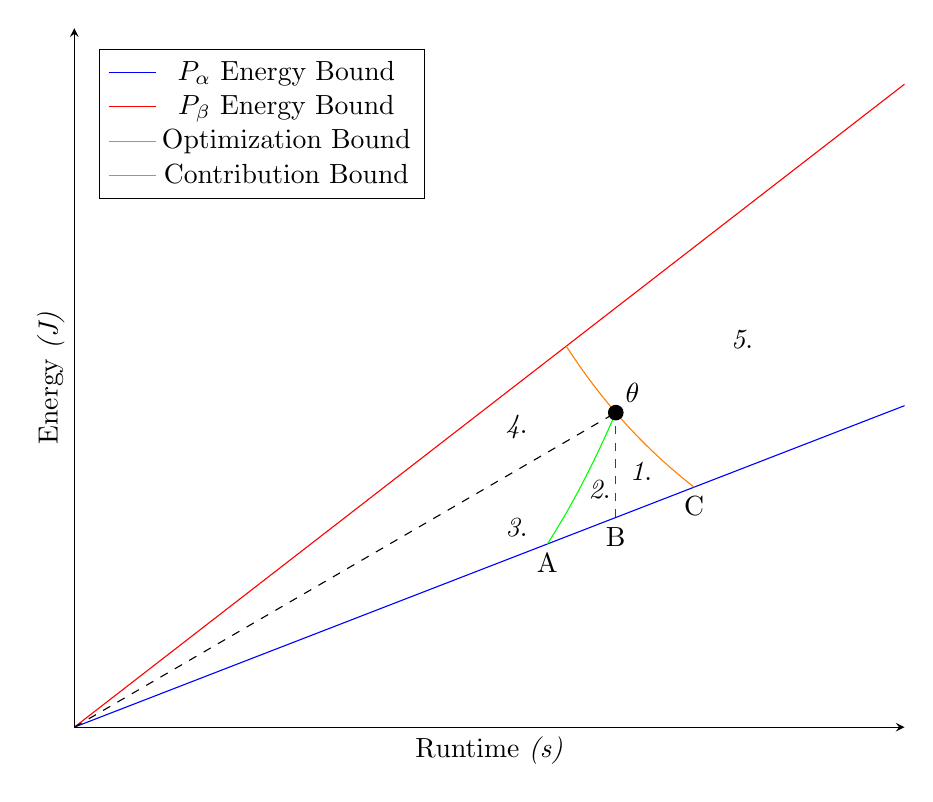
\begin{tikzpicture}
  \begin{axis}[ticks = none, 
    axis x line=bottom,axis y line=left,
ylabel={Energy \emph{(J)}}, xlabel={Runtime \emph{(s)}}, axis on top,
    ymin=0, ymax=3000,
    xmin=0, xmax=46,
    width=\linewidth,
    legend style={legend pos=north west}
    ]

    %% Model Parameters %%
    \pgfmathsetmacro{\baselinepower}{30} % NOP code
    \pgfmathsetmacro{\rooflinepower}{60}
    \pgfmathsetmacro{\codepower}{(\baselinepower + \rooflinepower) / 2}
    \pgfmathsetmacro{\codetime}{30}
    % Sadly, pgfplots sucks too much to calculate cube roots
    \pgfmathsetmacro{\anodex}{26.20741}
    \pgfmathsetmacro{\anodey}{\anodex * \baselinepower}
    \pgfmathsetmacro{\cnodex}{34.34143}
    \pgfmathsetmacro{\cnodey}{\cnodex * \baselinepower}
    \pgfmathsetmacro{\tnodex}{27.25681}
 
    %% Intermezzo Values %%
    \pgfmathsetmacro{\codeenergy}{\codepower * \codetime}
    \pgfmathsetmacro{\baselineenergy}{\baselinepower * \codetime}
    \pgfmathsetmacro{\rooflineenergy}{\rooflinepower * \codetime}
    \pgfmathsetmacro{\lowdisplayline}{(2 * \baselinepower + \codepower) / 3}
    \pgfmathsetmacro{\highdisplayline}{(1 * \rooflinepower + 1 * \codepower) / 2}

    % arguments: code power, code time, x - todo, apparently not supposed to do pgfmathparse
    \pgfmathdeclarefunction{metricbound}{3}{%
      \pgfmathparse{((#1 * #2^3) / #3^2)}%
    }
    \pgfmathdeclarefunction{definitionbound}{3}{%
      \pgfmathparse{((#1 / #2^3) * #3^4)}%
    }
     \pgfmathdeclarefunction{optimizationlimits}{3}{%
      \pgfmathparse{(min(metricbound(#1, #2, #3), definitionbound(#1, #2, #3)))}
    }

    % ALPHA BASELINE BOUND 
    \addplot[domain=\pgfkeysvalueof{/pgfplots/xmin}:\pgfkeysvalueof{/pgfplots/xmax},
             blue] {\baselinepower * x};
    \addlegendentry{$P_{\alpha}$ Energy Bound} 
    % BETA ROOFLINE BOUND
    \addplot[domain=\pgfkeysvalueof{/pgfplots/xmin}:\pgfkeysvalueof{/pgfplots/xmax},
             red] {\rooflinepower * x};
    \addlegendentry{$P_{\beta}$ Energy Bound} 

    % Constant Time and Power Dashes
    \draw[darkgray, dashed] ({axis cs:\codetime,\baselineenergy}) -- ({axis cs:\codetime,\codeenergy});
    \draw[dashed] ({axis cs:\pgfkeysvalueof{/pgfplots/xmin},\pgfkeysvalueof{/pgfplots/ymin}}) -- ({axis cs:\codetime,\codeenergy});
 

    \addplot[domain=\tnodex:\cnodex, orange] { metricbound(\codepower, \codetime, x)};
    \addlegendentry{Optimization Bound}

    \addplot[domain=\anodex:\codetime, green] { definitionbound(\codepower, \codetime, x)};
    \addlegendentry{Contribution Bound}


    \node[circle,fill,inner sep=2pt] at (axis cs:\codetime,\codeenergy) {};
    \node[above right] at (axis cs:\codetime,\codeenergy) {$\theta$};
    \pgfmathsetmacro{\oneycoord}{\lowdisplayline * 31.4}
    \node at (axis cs:31.4,\oneycoord) {\textit1.};
    \pgfmathsetmacro{\twoycoord}{\lowdisplayline * 29.1}
    \node at (axis cs:29.1,\twoycoord) {\textit2.};
    \pgfmathsetmacro{\threeycoord}{\lowdisplayline * 24.5}
    \node at (axis cs:24.5,\threeycoord) {\textit3.};
    \pgfmathsetmacro{\fourycoord}{\highdisplayline * 24.5}
    \node at (axis cs:24.5,\fourycoord) {\textit4.};
    \pgfmathsetmacro{\fiveycoord}{\codepower * 37}
    \node at (axis cs:37,\fiveycoord) {\textit5.};
    
    \node [below] at ({axis cs:\anodex, \anodey}) {A};
    \node [below] at ({axis cs:\codetime,\baselineenergy}) {B};
    \node [below] at ({axis cs:\cnodex, \cnodey}) {C};
    %\node [below, name intersections={of=metric bound and baseline}] at (intersection-1) {C};


 \end{axis}
\end{tikzpicture}

\caption{$ED^2P$ Code Optimization Space}\label{fig:modeldraw}
\end{figure}


The bounds presented above allow us to identify the area in the Energy/Runtime plane where power-optimized versions of a given code may exist. For the purposes of illustration we add lines of fixed time and power draw based on our initial code measurement. This allows us to subdivide \figurename~\ref{fig:modeldraw} into those areas labelled:

\begin{enumerate}
\centering
\item Power-only optimizations
\item Power-mostly optimizations
\item Time-mostly optimizations
\item Time-only optimizations
\item Code degradation
\end{enumerate}

Only three measurements are required to build this plot; the system's baseline power draw, $P_\alpha$, and the time and energy to solution for the code to be optimized, $D_\theta$ and $E_\theta$ respectively. We can ignore the value of $P_\beta$ when optimizing for power draw as we need not consider any values greater than our initial $P_\theta$.

Despite its simplicity, this technique offers a surprising wealth of information. The vertical distance between $\theta$ and intercept $B$ places an upper limit on the absolute amount of energy which can be saved by power optimization alone. The value $M(\theta) / M(A)$ bounds the amount of improvement in our metric we can expect to see from power optimization. The difference in runtime between intersect $C$ and $\theta$ represents the amount of time we are able to trade off if we hope to achieve a slower yet more energy efficient code. Finally, the value $D(\theta) / D(A)$ represents the smallest speed-up which delivers more benefit than power optimization is capable of.

At this point it is worth stating explicitly that our heuristic is a general one. Its only requirements are that power consumption is proportional to activity factor and that energy and time figures can be obtained for the system baseline and the code under investigation. As such it can be applied equally well at scales ranging from a single core to an entire system. We focus on CPU power consumption simply because measurements are relatively easy to obtain at this level.

We set out to apply our technique to a number of HPC benchmarks. Our first task was to measure the $P_\alpha$ baseline for our test system. This machine incorporates a commodity Intel Ivy Bridge processor which exposes the Running Average Power Limit interface \cite{david:2010aa}. For this reason we chose to use the techniques outlined in \cite{hackenberg:2013aa} to perform our measurements. This choice was made primarily out of convenience, as our method does not rely on any particular hardware or measurement configurations. The only prerequisites are that the system under test is CMOS-based and accurate power and time measurements are available.

\begin{table}
\centering
\small
\begin{tabular}{@{}ccccc@{}} \toprule
&\multicolumn{4}{c}{CPU Cores Active} \\ \cmidrule(r){2-5}
Frequency (GHz) & 1 & 2 & 3 & 4 \\ \midrule 
1.60 & 9.180 & 10.970 & 12.832 & 14.555 \\ 
1.70 & 9.449 & 11.446 & 13.295 & 15.112 \\ 
1.80 & 9.592 & 11.654 & 13.617 & 15.682 \\ 
1.90 & 9.816 & 12.009 & 14.168 & 16.291 \\ 
2.10 & 10.272 & 12.709 & 15.161 & 17.605 \\ 
2.20 & 10.559 & 13.161 & 15.705 & 18.333 \\ 
2.30 & 10.812 & 13.551 & 16.419 & 19.070 \\ 
2.40 & 11.303 & 14.290 & 17.012 & 19.946 \\ 
2.50 & 11.680 & 14.784 & 18.000 & 20.837 \\ 
2.60 & 11.819 & 15.144 & 18.616 & 21.879 \\ 
2.70 & 12.205 & 15.830 & 19.379 & 22.940 \\ 
2.90 & 13.095 & 17.196 & 21.155 & 25.344 \\ 
3.00 & 13.547 & 18.160 & 22.210 & 26.759 \\ 
3.10 & 14.048 & 18.870 & 23.639 & 28.284 \\ 
3.20 & 14.504 & 19.726 & 24.940 & 29.857 \\ 
\bottomrule
\end{tabular}
   \vspace{0.5\baselineskip}
\caption{Test Platform Base CPU Power (W)}
\label{tab:baseline}
\end{table} 

We measured CPU power draw whilst running our baseline micro-benchmark for each combination of core count and frequency which was supported by the hardware of our test platform. The results of this investigation are given in Table \ref{tab:baseline}. We then ran a range of codes chosen from common benchmarking suites, targeting various core counts and system configurations. A small number of results from the Rodinia suite is presented in Table \ref{tab:coderesults}. These results come from runs which were configured to use the maximum frequency and core count possible. Our baseline power draw for this configuration is 29.857 Watts.


\begin{table}
\centering
\small
\begin{tabular}{@{}ccccc@{}} \toprule
Code & Runtime (s) & Energy (J) & Power (W) & $ED^2P$ \\ \midrule 
CFD & 29.72 & 933.32 & 31.40 & 824381  \\ 
Heartwall & 24.62 & 787.17 & 31.97 & 477139 \\ 
lavaMD & 66.18 & 2142.65 & 32.38 & 9384362\\ 
leukocyte &  38.92 & 1197.91 & 30.78 & 1814554 \\ 
streamcluster & 33.86 & 1086.77 & 32.10 & 1245981 \\ 
\bottomrule
\end{tabular}
   \vspace{0.5\baselineskip}
\caption{Rodinia Results @ 3.2GHz, 4 Cores}
\label{tab:coderesults}
\end{table} 

Of the codes listed above, lavaMD is the strongest candidate for optimization as it has both the highest power draw at 32.38 Watts and the longest runtime of 66.18s. Applying our heuristic to this code yields the optimization space shown in \figurename~\ref{fig:lavamd}. This construction allows us to derive a number of additional metrics, as described below.


\begin{figure}
 
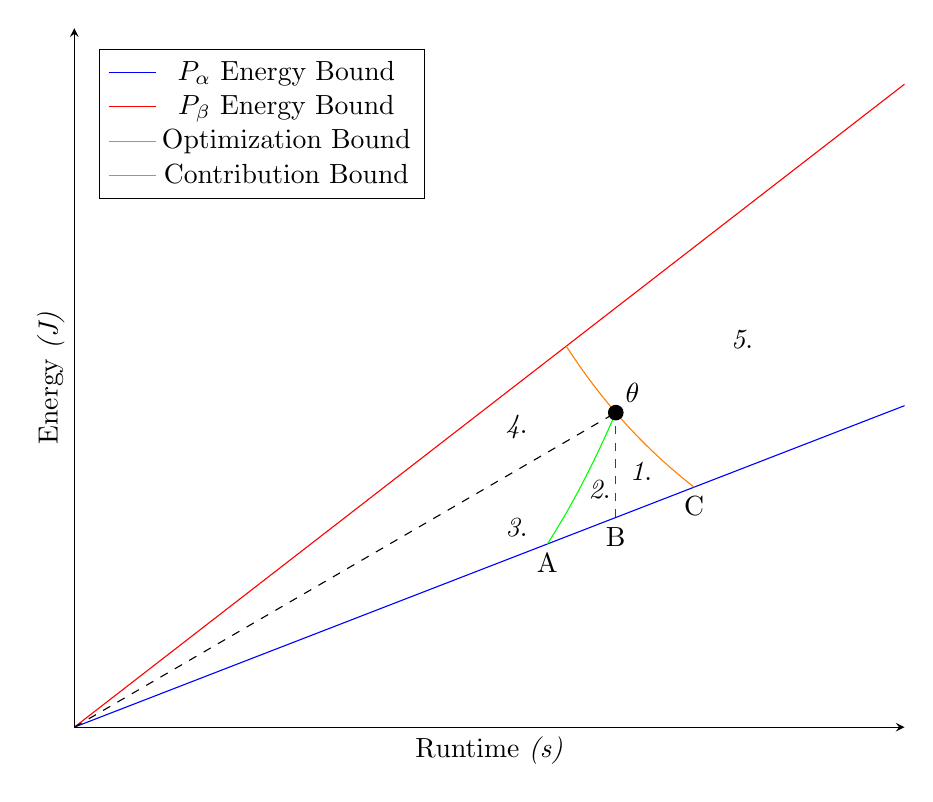
\begin{tikzpicture}
  \begin{axis}[ticks = none, 
    axis x line=bottom,axis y line=left,
ylabel={Energy \emph{(J)}}, xlabel={Runtime \emph{(s)}}, axis on top,
    ymin=0, ymax=3000,
    xmin=0, xmax=46,
    width=\linewidth,
    legend style={legend pos=north west}
    ]

    %% Model Parameters %%
    \pgfmathsetmacro{\baselinepower}{30} % NOP code
    \pgfmathsetmacro{\rooflinepower}{60}
    \pgfmathsetmacro{\codepower}{(\baselinepower + \rooflinepower) / 2}
    \pgfmathsetmacro{\codetime}{30}
    % Sadly, pgfplots sucks too much to calculate cube roots
    \pgfmathsetmacro{\anodex}{26.20741}
    \pgfmathsetmacro{\anodey}{\anodex * \baselinepower}
    \pgfmathsetmacro{\cnodex}{34.34143}
    \pgfmathsetmacro{\cnodey}{\cnodex * \baselinepower}
    \pgfmathsetmacro{\tnodex}{27.25681}
 
    %% Intermezzo Values %%
    \pgfmathsetmacro{\codeenergy}{\codepower * \codetime}
    \pgfmathsetmacro{\baselineenergy}{\baselinepower * \codetime}
    \pgfmathsetmacro{\rooflineenergy}{\rooflinepower * \codetime}
    \pgfmathsetmacro{\lowdisplayline}{(2 * \baselinepower + \codepower) / 3}
    \pgfmathsetmacro{\highdisplayline}{(1 * \rooflinepower + 1 * \codepower) / 2}

    % arguments: code power, code time, x - todo, apparently not supposed to do pgfmathparse
    \pgfmathdeclarefunction{metricbound}{3}{%
      \pgfmathparse{((#1 * #2^3) / #3^2)}%
    }
    \pgfmathdeclarefunction{definitionbound}{3}{%
      \pgfmathparse{((#1 / #2^3) * #3^4)}%
    }
     \pgfmathdeclarefunction{optimizationlimits}{3}{%
      \pgfmathparse{(min(metricbound(#1, #2, #3), definitionbound(#1, #2, #3)))}
    }

    % ALPHA BASELINE BOUND 
    \addplot[domain=\pgfkeysvalueof{/pgfplots/xmin}:\pgfkeysvalueof{/pgfplots/xmax},
             blue] {\baselinepower * x};
    \addlegendentry{$P_{\alpha}$ Energy Bound} 
    % BETA ROOFLINE BOUND
    \addplot[domain=\pgfkeysvalueof{/pgfplots/xmin}:\pgfkeysvalueof{/pgfplots/xmax},
             red] {\rooflinepower * x};
    \addlegendentry{$P_{\beta}$ Energy Bound} 

    % Constant Time and Power Dashes
    \draw[darkgray, dashed] ({axis cs:\codetime,\baselineenergy}) -- ({axis cs:\codetime,\codeenergy});
    \draw[dashed] ({axis cs:\pgfkeysvalueof{/pgfplots/xmin},\pgfkeysvalueof{/pgfplots/ymin}}) -- ({axis cs:\codetime,\codeenergy});
 

    \addplot[domain=\tnodex:\cnodex, orange] { metricbound(\codepower, \codetime, x)};
    \addlegendentry{Optimization Bound}

    \addplot[domain=\anodex:\codetime, green] { definitionbound(\codepower, \codetime, x)};
    \addlegendentry{Contribution Bound}


    \node[circle,fill,inner sep=2pt] at (axis cs:\codetime,\codeenergy) {};
    \node[above right] at (axis cs:\codetime,\codeenergy) {$\theta$};
    \pgfmathsetmacro{\oneycoord}{\lowdisplayline * 31.4}
    \node at (axis cs:31.4,\oneycoord) {\textit1.};
    \pgfmathsetmacro{\twoycoord}{\lowdisplayline * 29.1}
    \node at (axis cs:29.1,\twoycoord) {\textit2.};
    \pgfmathsetmacro{\threeycoord}{\lowdisplayline * 24.5}
    \node at (axis cs:24.5,\threeycoord) {\textit3.};
    \pgfmathsetmacro{\fourycoord}{\highdisplayline * 24.5}
    \node at (axis cs:24.5,\fourycoord) {\textit4.};
    \pgfmathsetmacro{\fiveycoord}{\codepower * 37}
    \node at (axis cs:37,\fiveycoord) {\textit5.};
    
    \node [below] at ({axis cs:\anodex, \anodey}) {A};
    \node [below] at ({axis cs:\codetime,\baselineenergy}) {B};
    \node [below] at ({axis cs:\cnodex, \cnodey}) {C};
    %\node [below, name intersections={of=metric bound and baseline}] at (intersection-1) {C};


 \end{axis}
\end{tikzpicture}

\caption{Power Heuristic for Rodinia lavaMD} \label{fig:lavamd}
\end{figure}

If we assume it is somehow possible to reduce the activity factor of lavaMD to match that of our  micro-benchmark which performs no work, then the corresponding energy savings at point B would amount to 166.71 Joules, a $7.8\%$ reduction. This corresponds to an improvement in $ED^2P$ of $1.08\times$ from 9384362 to 8654190. Point A represents the most extreme case; reducing activity factor to the minimum possible whilst also significantly speeding up our code. This scenario yields an $ED^2P$ of 7979856, an improvement of $1.17\times$.

For lavaMD, the longest runtime within our optimization envelope is 69.99s. This means that any power optimization which seeks to trade increased runtime for improved energy efficiency can slow lavaMD down by at most 1.81s before $ED^2P$ becomes strictly worse. Furthermore, we know the fastest out code can run whilst remaining in our envelope is 64.41s. This means that a classical optimization which reduces runtime by 1.77s or more is strictly better than all valid power optimizations at minimizing $ED^2P$. A modest $1.03\times$ speed-up from classical optimization yields more benefit than any power optimization ever could.

The figures listed above are all upper bounds which could not be achieved in reality. The true benefits of power optimization are likely to be significantly more modest in practice. Even so, these figures are worthwhile as they allow performance engineers to make an informed decision about where best to focus their efforts. If they consider a $1.03 \times$ speed up to be more readily achievable than a significant reduction in activity factor then they can proceed to apply conventional optimizations safe in the knowledge that energy consumption will reduce regardless of whether they increase the activity factor or not. On the other hand, if no runtime improvements are forthcoming, then power optimization techniques may still be able to find improvements where traditional approaches have failed.


If a performance engineer decides the benefits of power optimization are worth pursuing after applying the test outlined above, the question still remains as to how he should go about searching for those optimizations. Conventional tools produce a breakdown of time spent by code path by halting the target application at timed intervals and recording its state. By extension, a sampling profiler which operated in intervals of energy instead of time it would show the contribution of different code sections to total energy use.

We first construct a power model in the vein of those proposed in the literature. We then try to link the predictions of our model to the power equations given previously. Essentially we are attempting to test against the null hypothesis - to show how much better or worse our regressed model is better than a naive attempt.



\fragment{Often power models are assessed by their performance relative to a measured baseline. Although this is important, this figure is somewhat meaningless without context. Our approach is one of quantifying 


\todo{Make this bit less attacky:}
It is also worth noting that this model is effectively useless from a code optimization standpoint as it does not take any software features into account. This property is intentional, as it allows us once again to provide a baseline from which to assess any models. One can only realistically expect to optimize a code to the level at which any changes can be accurately measured. A model which claims to assist in the optimization of codes can only offer optimizations to the extent it shows divergence from this baseline.

}


\fragment{The unknown quantities in our simplified power equations can be empirically measured. \todo{Occam's razor - stronger than regression if not out performed by it}}



\fragment{Accuracy figures without context are notoriously unreliable. To compensate for this we compare the outputs of various models against a baseline we have devised. This baseline consists of what we regard as the simplest non-trivial power model conceivable. This model stands in as a sort of null hypothesis test, our justification being that a complex model only adds value to the extent with which it outperforms this toy model.}

\fragment{Our toy model is not the simplest model possible - It is well established and readily apparent that runtime is the largest contributory factor to power consumption. One could therefore imagine a simple power model}

\fragment{We consider this to be the absolute minimum power consumption possible.}

\fragment{Intentionally simplistic. Our decision to simplify activity factor to active cores is part of this. We assume that instruction pipe-lining does a reasonable job of keeping as much silicon active as possible, and we do not know how much area an individual instruction activates, and a large percentage of power use is from clock circuitry anyway}




\todo{Be nice, say that this does not invalidate other work, but simply shows that hardware has now reached \reword{convergence} and basically there's little traction left}

Having shown that 

\fragment{This model is not supposed to be rigorous or precise. Rather we present it as the simplest possible non-trivial power model which accounts for the sources of variability in the power equations. In effect our model is functionally equivalent to the power equations
presented previously with appropriate constants substituted \todo{sampled}. We present this model as our null hypothesis - for a model to be useful it must outperform this one. It is necessarily an oversimplification - it ignores clock gating. It should also consistently underestimate the true value, as the benchmark selected intentionally exercises the minimum possible number of logic elements while still performing work.}


\todo{One limitation of this work stems from the nature of RAPL - it is an accumulative measurement of power taking into account all processes. On a loaded system it will measure all tasks }

\begin{figure}
\label{fig:dummy_model}
\includegraphics[width=0.9\linewidth]{./Plots/dummy_model/dummymodel-figure0.pdf}
\caption{Feasible Performance Envelope}
\end{figure}

\todo{Decompose the model - find baseline vs non-baseline components}
\todo{This kind of shows us that the baseline dominates}

\fragment{Limitations to optimizations - the superfluous and the logical equivalences. The first is a no-brainer and boils down to removing unnecessary pre-fetching}

\fragment{Either optimizations which are off the critical path, or else those which are on the critical path }


\todo{Do maths think - by what margin would power have to go down to justify longer runtime? ratio of cost per watt, amortized cost per second}

Nothing discussed so far precludes power optimization in practice.
\todo{imply limits thus far are theoretical}
Even these tight limits may still admit some benefits at extreme scale.
Our final argument however is strictly economic.
\reword{A great deal of attention is paid to the fact that power costs are approaching parity with machine construction costs.} The \choice{implicit, unspoken} \choice{consequence, corollary, implication} being that this has not yet happened. \todo{Ultimate point being here the price difference, machine vs power cost places a further limit on optimization utility. Even if we manage to find a slower, more power efficient method of computing a given result, the cost of energy saved has to be less than the added amortized runtime cost.}


\todo{Legitimate targets for optimization: removing redundant prefetch operations as per phi paper.}

\section{Results}
\label{sec:results}
Present a series of limits on the potential gains from optimization.

\begin{itemize}
	\item The loosest limit we can impose is the fact that static power will be around. If somehow we reduce the activity factor of some workload, we will get at best x\% improvement.
	\item that's not so meaningful, and a large amount of the activity factor comes simply from clock circuits and whatnot. So we extrapolate this base from our power data, and basically power(0)..power(4) is our feasible range. See diagramx
	\item Ignoring blocking IO the critical path of a program takes x cycles. Assume fixed, non-fixed times. Power per cycle @ various frequencies.
\end{itemize}

\todo{Diagramx: Plot showing how clock circuitry dominates functional circuitry. We perform the same amount of work per cycle, but we either do [1..4] instructions on 1 core or 1 instruction on [1..4] cores. Expect two lines diverging. As each core comes on stream we see the clock circuitry and other supporting stuff cause steps.}
\section{Review of Prior Art}
\label{sec:prior}

In this section we detail work which attempts to assess the impacts of software on power consumption. Needless to say this work would form the basis of any attempt at software-level power optimization and as such warrants our scrutiny. A wealth of material also exists on architecture-level power optimizations, however this is outside the scope of our study.

\todo{To be able to optimize you need to be able to find}

\todo{taxonomy}

\begin{table}[ht]
  \begin{tabular}{|c|c|c|c|}
    \cline{3-4}
    \multicolumn{2}{c|}{} & \multicolumn{2}{c|} {Intrinsic Energy Characteristics} \\ \cline{3-4}
    
    \multicolumn{2}{c|}{} & Architecture Level & Instruction Level \\ \hline
    
      \multirow{6}{*}{\parbox[t]{1.4cm}{Activity\\Factor}} & \multirow{2}{*}{Simulator/Profiler} & Y & Z \\ \cline{3-4}
                                    & & Y & Z \\ \cline{2-4}
                                    & \multirow{2}{*}{Performance Counters} & Y & Z \\ \cline{3-4}
                                    & & Y & Z \\ \cline{2-4}
                                    & \multirow{2}{*}{Analytical Performance Model} & Y & Z \\ \cline{3-4}
                                    & & Y & Z \\ \hline

  \end{tabular}
  \caption{Energy Modelling Taxonomy}
  \label{table:taxonomy}
\end{table}


\todo{tear this apart: Energy Measurement and Prediction for Multi-threaded Programs}


\todo{
\begin{itemize}
\item Measurement vs modelling
\item Power is the integral and hard to measure
\item Approaches to measurement
\item Modelling taxonomy
\end{itemize}
}


\todo{Make sure to make the point that the accuracy quoted for models hovers around the same amount and is usually quoted as a simple average. There are several problems with such a figure. The simplest issue is that if a model can both over- and under-estimate, a low average error can be observed even when individual predictions are way off. If we give the authors the benefit of the doubt and assume they are reporting mean absolute error values. Even then, this methodology is somewhat flawed. To state a model yields an average error of 5\% does not necessarily display how good a model is. The nature of power, with both static and dynamic components along with known bounds means that reasonable guesses to power draw can be made a-priori. Any model constructed only has merit in as much as it beats these naive predictions.} 
\section{Conclusions}

\todo{IN an intuitive sense the covariance between these two signals, namely power and time consumption, is prohibitively high. The window of optimization exists in the ...word meaning freedom/decoupled component/... window}

\section{Notes}

\todo{\begin{enumerate}
\item Merge this delta section - use for snippets
\item Consider moving Code optimization out of intro
\item Optimizable range is only a small part of this part
\item Write a clear limitations section

\end{enumerate}
}



\todo{Say how the baseline does not include halts, but halted states are time dependent only }
\begin{figure}
\label{fig:tlpilp}
\includegraphics[width=0.9\linewidth]{./Plots/tlp_vs_ilp/tlpilp-figure0.pdf}
\caption{Power Overhead from TLP and ILP}
\end{figure}

\todo{Make comment about how reducing the activity factor is in some sense counter to time optimization - that doing more per unit time is better. }


\todo{Energy Measurement and Prediction for Multi-threaded Programs -- this gives a simple model based on power modelling and claims sub 10 \%}


\todo{citation S. Kaxiras and M. Martonosi, Computer Architecture Techniques for Power-Efficiency, 1st ed. Morgan and
Claypool Publishers, 2008.

The end of Dennard scaling is expected to shrink the range of DVFS in future nodes, limiting the energy savings of this technique. This paper evaluates how much we can increase the effectiveness of DVFS by using a software decoupled access-execute approach. Decoupling the data access from execution allows us to apply optimal voltage-frequency selection for each phase and therefore improve energy efficiency over standard coupled execution.
}
\todo{Cite this paper for dennard: A 30 Year Retrospective on Dennard's MOSFET Scaling Paper}

\reword{Dennard scaling, which roughly, that as transistors get smaller their power density stays constant, so that the power use stays in proportion with area: both voltage and current scale (downward) with length \todo{cite Dennard's paper}}

\fragment{When viewed in this context, all event-driven power models are simply linking performance events back to their associated activity costs/factors}


\reword{The uncore is a collection of components of a processor
not in the core but essential for core performance. The
CPU core contains components involved in executing in-
structions, including execution units, L1 and L2 cache,
branch prediction logic, etc. Uncore functions include
the last level cache (LLC), integrated memory controllers
(IMC), on-chip interconnect (OCI), power control logic
(PWR), etc. as shown in Figure 1. With growing cache
sizes and the integration of various SoC components on
CPU die, the uncore is becoming an increasingly impor-
tant contributor to total SoC power.}









\todo{PMB2014 checkpointing paper - exascale expects 70\% of energy to go to memory dimms.}









\todo{PMBS2014 checkpointing paper 2 - extreme low or high frequency higher failure rate per job.}

\todo{Destroy this: Models and Metrics to Enable Energy-Efficiency Optimizations}







%\begin{table}
%\centering
%\small
%\begin{tabular}{@{}lll@{}} \toprule
%&\multicolumn{2}{c}{Granularity} \\ \cmidrule(r){2-3}
%Approach & Instruction Level & Architecture Level \\ %\midrule
%Measurement & Hanhel et. al.~\cite{hahnel:2012aa}  & %\todo{find eg}\\
%Perf. Counters & Shao \& Brooks~\cite{shao:2013aa} & %Isci \& Martonosi~\cite{isci:2003aa} \\
%Simulation &  Tiwari et. al.~\cite{tiwari:1994aa} & Li et. al.~\cite{li:2009aa} \\
%Analytical Modelling & Hong et. al.~\cite{hong:2010aa} %& Karkhanis \& Smith~\cite{karkhanis:2007aa} \\
%\bottomrule
%\end{tabular}
 % \caption{Energy Estimation Taxonomy}
  %\label{tab:taxonomy}
%d\end{table}








 
% TODO should be an IEEE bibstyle or something
% Left because we don't know requisite format yet, but ho hum
\bibliographystyle{plain}
\bibliography{library}


\end{document}